\section{Framework}

We present \framework, a comprehensive framework for evaluating agent reasoning in embodied tasks. Our framework addresses the fundamental challenge of assessing whether language models understand embodied principles. We achieve this through three key design principles: (1) tasks must require reasoning about physical properties and constraints rather than following explicit instructions, (2) agent capabilities should dynamically evolve based on tool acquisition rather than remaining static, and (3) collaboration needs should emerge from task requirements rather than predetermined protocols.

\subsection{Task Design and Formalization}

\paragraph{Environment Representation.}
We formalize embodied environments as directed graphs $G_t = (V_t, E_t, A_t)$ that capture the essential structure of physical spaces. The node set $V_t$ encompasses three entity types: spatial nodes representing rooms and areas, object nodes for interactive items, and agent nodes for autonomous entities. Each node maintains an attribute dictionary $A_t$ storing continuous physical properties such as weight, temperature, material composition, and geometric dimensions. The edge set $E_t$ encodes spatial relationships through static containment relations (e.g., ``in'', ``on'') and dynamic proximity relations $E_{\text{near}}$ that track which objects fall within an agent's interaction range. This graph representation enables efficient reasoning about spatial constraints while avoiding the computational overhead of continuous 3D simulation.

\paragraph{Task Formalization.}
Each evaluation task is defined as a tuple $\mathcal{T} = (S_{\text{init}}, I, G_{\text{goal}}, \mathcal{A}_{\text{task}})$, where $S_{\text{init}}$ specifies the initial environment state, $I$ provides the natural language instruction, $G_{\text{goal}}$ defines success conditions through logical predicates, and $\mathcal{A}_{\text{task}}$ identifies participating agents. The evaluation objective is to assess whether agents can generate an action sequence $\Pi = (\pi_1, \ldots, \pi_T)$ that transforms the environment from $S_{\text{init}}$ to a terminal state $S_{\text{final}}$ satisfying all predicates in $G_{\text{goal}}$. This formalization captures both the planning and execution aspects of embodied reasoning.

\subsection{Hierarchical Task Taxonomy}

Our evaluation framework organizes tasks along two orthogonal dimensions: agent configuration (single vs. multi-agent) and cognitive complexity (L1: basic, L2: intermediate, L3: advanced). This structure enables systematic assessment of how reasoning capabilities scale with task demands.

\paragraph{Single-Agent Tasks.}
Single-agent scenarios ($|\mathcal{A}_{\text{task}}| = 1$) isolate individual reasoning capabilities across three complexity levels. At the basic level, \textbf{\textit{Direct Command}} tasks require straightforward instruction following, such as ``place cup\#1 on table\#1,'' establishing baseline comprehension abilities. Intermediate complexity introduces two parallel challenges: \textbf{\textit{Attribute Reasoning}} tasks require comparing continuous properties to identify targets (e.g., ``move the heaviest cup'' requires solving $v^* = \arg\max_{v \in V_{\text{cups}}} A_t(v, \text{weight})$), while \textbf{\textit{Tool Use}} tasks demand recognizing capability gaps and acquiring right tools. For instance, ``clean the table'' requires agents to identify that cleaning actions are unavailable in their base action set $\mathcal{A}_i$, locate cleaning tools, and execute $\texttt{grasp}(v_{\text{tool}})$ to dynamically expand their capabilities. Advanced \textbf{\textit{Compound Reasoning}} tasks integrate multiple challenges, such as ``clean the heaviest table,'' requiring simultaneous attribute comparison, tool acquisition, and multi-step planning.

\paragraph{Multi-Agent Tasks.}
Multi-agent scenarios ($|\mathcal{A}_{\text{task}}| > 1$) evaluate coordination capabilities through parallel complexity progression. Basic \textbf{\textit{Explicit Collaboration}} tasks provide clear coordination directives, such as ``Agent A and Agent B cooperate to open the heavy cabinet,'' testing fundamental synchronization abilities. Intermediate \textbf{\textit{Implicit Collaboration}} removes explicit instructions, requiring agents to autonomously recognize when tasks exceed individual capabilities. For example, ``move the dining table to the storage room'' requires agents to infer that $A_t(v_{\text{table}}, \text{weight}) > C_{\max}(i)$ for any individual agent $i$, necessitating collaborative effort. Advanced \textbf{\textit{Compound Collaboration}} combines all elements, such as ``cooperatively repair the malfunctioning television,'' demanding tool acquisition, capability assessment, and coordinated execution.

\subsection{\simulator: Efficient Environment Simulation}

\paragraph{State Representation and Updates.}
\simulator employs text-based environment modeling to achieve efficient simulation at scale. The graph structure $G_t$ maintains spatial relationships through topological connections rather than continuous coordinates, eliminating expensive collision detection while preserving essential spatial constraints. State updates follow an incremental approach where actions modify only directly affected nodes and edges. For instance, when an agent executes $\texttt{GOTO}(\text{table})$, the system updates only the relevant proximity relations in $E_{\text{near}}$ rather than recomputing global spatial relationships.

\paragraph{Dynamic Capability Management.}
A key innovation in \simulator is the dynamic tool-capability binding system. Agent actions are partitioned into basic actions (movement, grasping, opening) available to all agents, and tool-dependent actions (cleaning, heating, repairing) that require specific tools. Each tool object maintains a \texttt{capability} attribute specifying which actions it enables. When an agent grasps a tool, the system dynamically binds the associated capabilities to the agent's action set. Upon releasing the tool, these capabilities are automatically unbound. This mechanism enables realistic modeling of how agents extend their abilities through tool use, moving beyond the static action spaces of existing benchmarks.

\paragraph{Emergent Collaboration.}
\simulator supports collaboration that emerges from physical constraints rather than explicit programming. When agents attempt actions on objects whose properties exceed individual capabilities, the system enables collaboration request mechanisms. For instance, if an agent attempts to move an object where $A_t(v, \text{weight}) > C_{\max}(\text{agent})$, it can initiate collaboration by identifying suitable partners and coordinating joint actions. The system validates preconditions for all participating agents and maintains consistency throughout collaborative execution, ensuring realistic multi-agent interactions.

\subsection{Automated Benchmark Generation}

\begin{figure*}
    \centering
    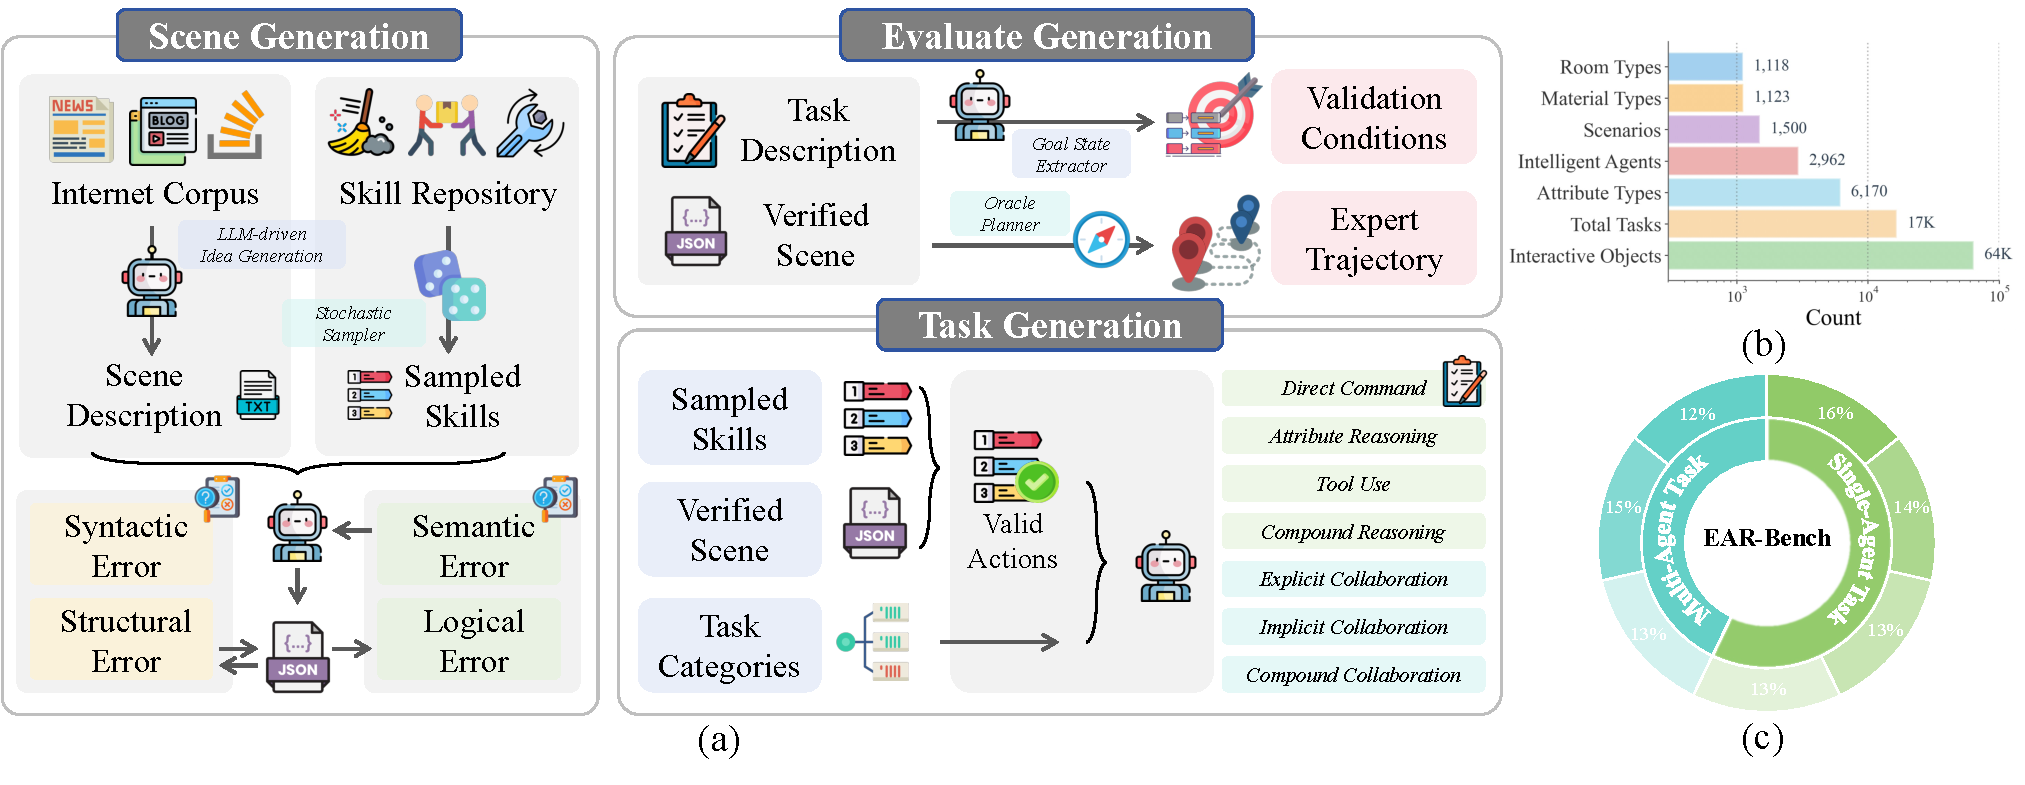
\includegraphics[width=1.0\textwidth,trim=0 13 0 0pt, clip]{figures/data_generation.pdf}
    \caption{OmniEAR automated benchmark generation and evaluation framework. (a) Four-stage generation pipeline combining LLMs with rule-based validation: scene generation from internet corpus, task generation with skill sampling, evaluation logic extraction, and expert trajectory generation with human validation. (b) EAR-Bench statistics: 1,500 scenarios, 64K objects, 6K attribute types, spanning diverse domains and material compositions. (c) Balanced task distribution across seven categories spanning single-agent (Direct Command, Tool Use, Attribute Reasoning, Compound Reasoning) and multi-agent tasks (Explicit/Implicit/Compound Collaboration).}
    \label{fig:data-generation-and-distribution}
\end{figure*}


\paragraph{Generation Pipeline.}
Creating diverse, physically consistent scenarios at scale requires careful orchestration of neural generation and symbolic validation. As shown in \ref{fig:data-generation-and-distribution}, our pipeline operates in four stages, each combining the creative capabilities of large language models with rule-based consistency checking. This hybrid approach enables generating thousands of unique scenarios while maintaining physical realism and task solvability.

\paragraph{Scene and Task Generation.}
Scene generation begins with semantic seeds extracted from diverse text sources\citep{li2024datacomp}, which guide a neural generator $g_{\text{scene}}$ in creating structured environment descriptions. The generator, implemented using high-temperature language models for diversity, produces initial scenes $S_0$ containing objects, spatial layouts, and agent configurations. Task generation follows a two-stage process: first, an environment analyzer $C_{\text{env}}$ extracts feasible actions based on the scene structure, then a task generator $g_{\text{task}}$ creates instructions anchored in physical possibilities. This grounding prevents generation of impossible tasks while maintaining creative diversity.

\paragraph{Evaluation Logic and Trajectories.}
For each generated task, we automatically derive evaluation criteria by parsing the instruction and scene to extract minimal state changes required for success. This produces a goal predicate set $G_{\text{goal}}$ that serves as an objective success measure. Expert trajectories are generated using oracle agents with complete environmental knowledge, creating high-quality demonstrations for each task. These trajectories undergo filtering to remove suboptimal sequences, providing ideal solutions for comparison and learning.

\paragraph{Quality Assurance.}
All generated content passes through multi-tier validation. Automated validators check structural consistency, physical feasibility, and logical coherence. Human evaluators then attempt to solve each task using our interactive interface, identifying subtle issues that automated checks miss. This human-in-the-loop process ensures that all tasks in \benchmark are both challenging and solvable, maintaining benchmark quality while achieving scale.

\subsection{Benchmark Statistics and Coverage}

\benchmark encompasses 1,500 scenarios across 11 domains including laboratory (39\%), office (19\%), industrial (12\%), and medical environments, containing 64,057 interactive objects with rich physical properties. The dataset maintains careful balance across our task taxonomy: 65\% single-agent tasks spanning all complexity levels, and 35\% multi-agent tasks with emphasis on implicit collaboration scenarios that require genuine reasoning about coordination needs. With 6,381 distinct property types and 214 action types, \benchmark provides comprehensive coverage of embodied reasoning challenges while maintaining tractable evaluation scope. Detailed statistics are provided in Appendix \ref{sec:dataset_statics}.

% \benchmark encompasses 1,500 scenarios across xx domains (household, office, industrial, and service, etc .), containing 64,057 interactive objects with rich physical properties. The dataset maintains careful balance across our task taxonomy: 65\% single-agent tasks spanning all complexity levels, and 35\% multi-agent tasks with emphasis on implicit collaboration scenarios that require genuine reasoning about coordination needs. With over 6,170 distinct property types and 200+ action types, \benchmark provides comprehensive coverage of embodied reasoning challenges while maintaining tractable evaluation scope. A comprehensive comparison with related work is provided in Appendix \ref{sec:dataset_statics}.

% \subsection{Benchmark Statistics and Coverage}

% \benchmark encompasses 1,500 scenarios across household, office, industrial, and service domains, containing 64,057 interactive objects with rich physical properties. As shown in Table~\ref{tab:dataset_statistics}, the dataset maintains careful balance across our task taxonomy: 65\% single-agent tasks spanning all complexity levels with equal representation (approximately 16.3\% each), and 35\% multi-agent tasks with emphasis on implicit collaboration scenarios (14\%) that require genuine reasoning about coordination needs. The benchmark features exceptional diversity with over 6,170 distinct property types enabling nuanced physical reasoning, 1,123 different materials supporting realistic constraint modeling, and 214 action types partitioned between basic actions (60\%) and tool-dependent actions (40\%). Each scenario includes expert demonstration trajectories averaging 8.7 steps, validated through human evaluation to ensure task solvability. This comprehensive coverage enables systematic evaluation of embodied reasoning capabilities while maintaining tractable evaluation scope.